\chapter{System Description}

Password managers are tools that stores all the users password in a single
vault or database, making it easier for a user with a lot of account to keep
track of their passwords and usernames. A password manager can also make it
more secure for the user, since they nudge the user to not reuse passwords.
This hoverer only is true if the password manager is sufficient secure itself.

The password manager in this assignment can have multiple users, that uses
multiple devices to access the password manager. \Cref{fig:sys:arch} shows the
architecture for the system. Here it can be seen how the system should be able
to serve multiple users. These users can access their account through the user
database.

Each account has an access manager. The access manager will check the user
against the user data; is the password correct, is the device authorized, ect.
Only if the access manager grants access to the account will it decrypt and
serve the password database to the user. The access manager also has the
responsibility to logout the user on timeout, and to authorize new devices when
the user wishes to access the database from a new device.

The password database is unique for each user, and can hold as many passwords
as the user wishes.

\begin{figure}[H]
    \centering
    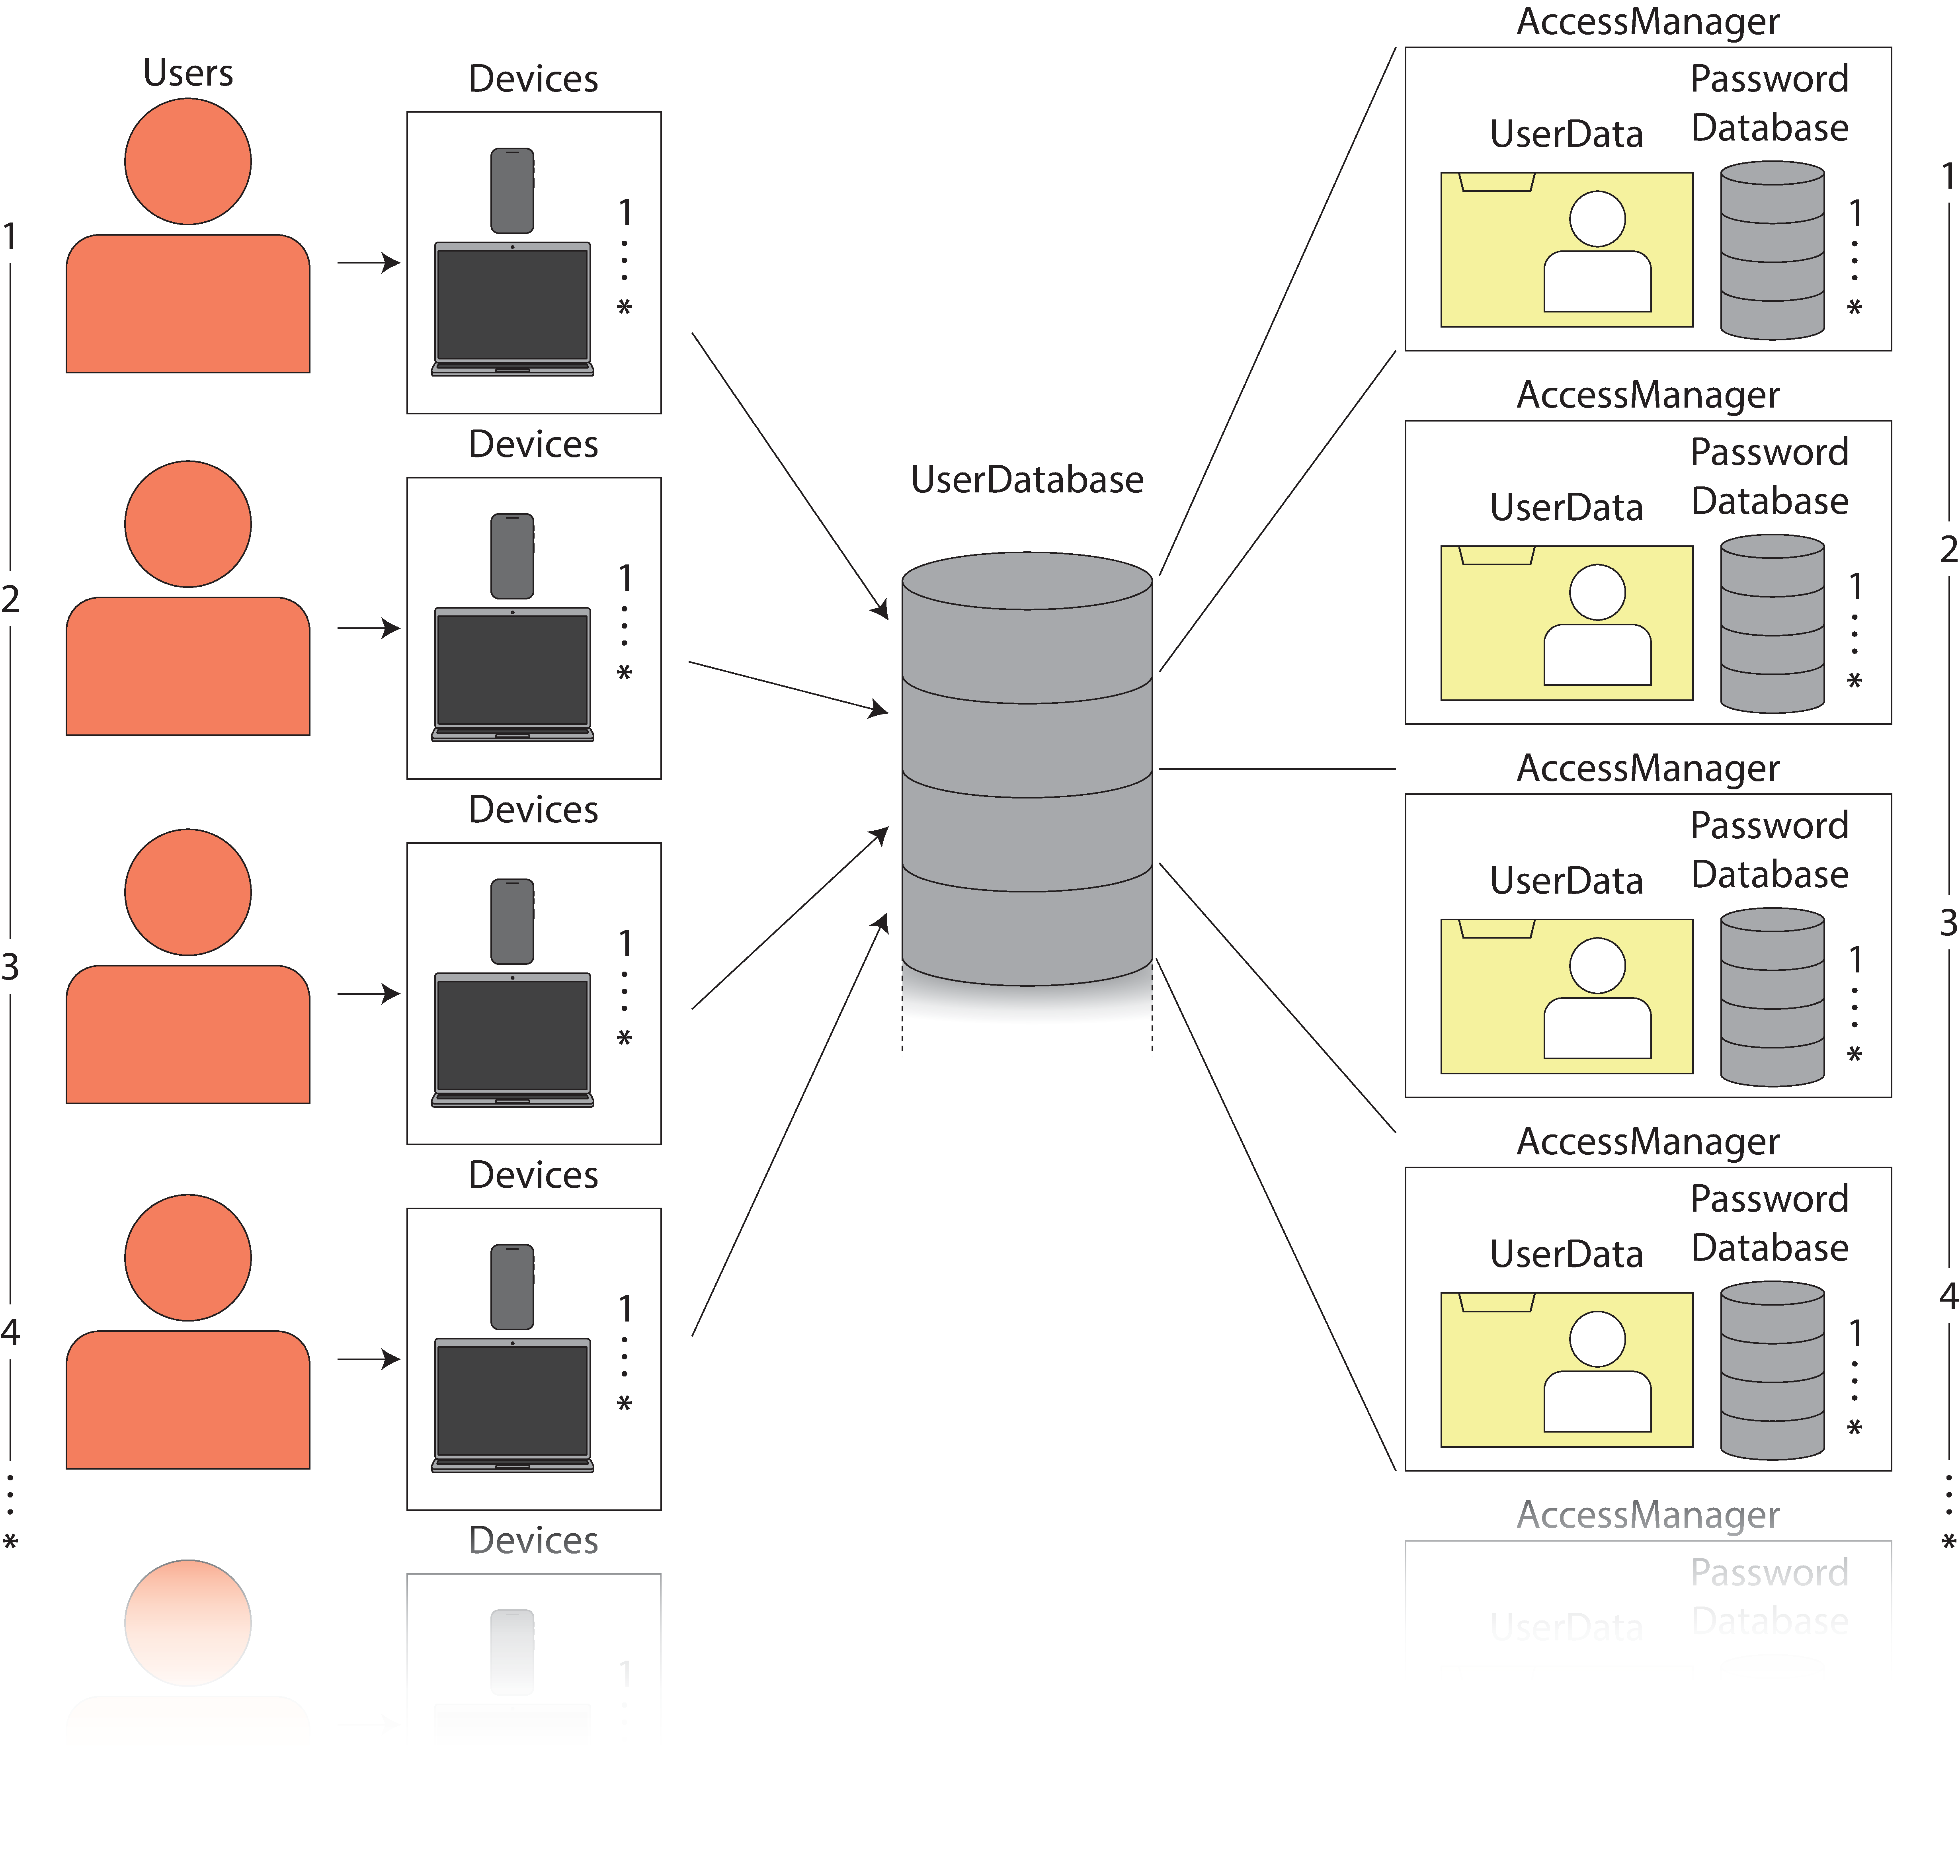
\includegraphics[width=\textwidth]{prj/figs/Architecture.pdf}
    \caption{Diagram over the architecture of the system.}
    \label{fig:sys:arch}
\end{figure}